\documentclass[12pt,a4paper]{article}
\usepackage[utf8]{inputenc}
\usepackage[T1]{fontenc}
\usepackage[polish]{babel}
\usepackage{amsmath}
\usepackage{amssymb}
\usepackage{geometry}
\usepackage{listings}
\usepackage{xcolor}
\usepackage{graphicx}
\usepackage{hyperref}
\usepackage{float}

\geometry{top=2.5cm, bottom=2.5cm, left=2.5cm, right=2.5cm}

% Konfiguracja listowania kodu dla języka Julia
\lstdefinelanguage{Julia}%
  {morekeywords={abstract,break,case,catch,const,continue,do,else,elseif,%
      end,export,false,for,function,immutable,import,importall,if,in,%
      macro,module,mustcontain,type,typealias,using,true,while,struct},%
   sensitive=true,%
   morecomment=[l]{\#},%
   morecomment=[s]{{\#=}}{={\#}},%
   morestring=[b]",%
   morestring=[m]'%
}[keywords,comments,strings]

\lstset{
    language=Julia,
    backgroundcolor=\color{gray!5},
    basicstyle=\small\ttfamily,
    keywordstyle=\color{blue}\bfseries,
    commentstyle=\color{green!50!darkgray}\italicshape,
    stringstyle=\color{purple},
    numbers=left,
    numberstyle=\tiny\color{gray},
    stepnumber=1,
    numbersep=8pt,
    frame=single,
    rulecolor=\color{gray!30},
    breaklines=true,
    captionpos=b
}

\title{\textbf{Sprawozdanie 3}\\Wybrane Zagadnienia Algebry}
\author{Jakub Kowal\\279706}
\date{}

\begin{document}

\maketitle

\section{Wstęp i implementacja pierścieni wielomianów wielu zmiennych}

\subsection{Różnice w implementacji względem wielomianów jednej zmiennej}
Implementacja pierścienia wielomianów wielu zmiennych $R[x_1, \dots, x_n]$ wykazuje istotne różnice strukturalne i algorytmiczne w porównaniu do wielomianów jednej zmiennej:
\begin{itemize}
    \item \textbf{Reprezentacja wykładników:} W przypadku jednej zmiennej wykładnik jednomianu reprezentowany jest przez pojedynczą liczbę całkowitą (klucz w słowniku lub indeks w tablicy). W wielu zmiennych konieczne jest zastosowanie wektora liczb całkowitych ($\mathtt{Vector\{Int\}}$), gdzie każdy element odpowiada potędze przypisanej do konkretnej zmiennej (np. wektor $[2, 1, 0]$ oznacza $x_1^2 x_2^1 x_3^0$).
    \item \textbf{Porządek jednomianów (Monomial Order):} Dla jednej zmiennej relacja porządku jest trywialna (wyższy stopień dominuje). W przestrzeni wielowymiarowej nie istnieje jeden naturalny porządek. Wymaga to jawnego zdefiniowania relacji takich jak porządek leksykograficzny ($\mathtt{LexOrder}$) czy stopniowany leksykograficzny ($\mathtt{GradedLexOrder}$), które są kluczowe dla jednoznacznego wyznaczenia wyrazu wiodącego ($\mathtt{leading\_term}$).
    \item \textbf{Zgodność wymiarów:} Struktura wielomianu wielu zmiennych musi jawnie przechowywać informację o liczbie obsługiwanych zmiennych ($\mathtt{nvars}$), aby uniemożliwić błędy semantyczne podczas dodawania lub mnożenia obiektów należących do różnych przestrzeni.
\end{itemize}

\section{Zaimplementowane algorytmy}

Poniżej przedstawiono kody źródłowe kluczowych operacji algebraicznych zrealizowanych w języku Julia, stanowiących rozszerzenie dostarczonej biblioteki bazowej.

\subsection{S-wielomian (Syzygium)}
S-wielomian służy do eliminacji wyrazów wiodących pary wielomianów w celu wyszukiwania nowych relacji w ideale.
\begin{lstlisting}[caption={Implementacja wyznaczania S-wielomianu}]
function lcm_exp(e1::Vector{Int}, e2::Vector{Int})
    return max.(e1, e2)
end

function Syzygium(f::Wielomian{T}, g::Wielomian{T}, order::MonomialOrder) where T
    e_f, c_f = leading_term(f, order)
    e_g, c_g = leading_term(g, order)
    
    e_lcm = lcm_exp(e_f, e_g)
    
    exp_mult_f = e_lcm .- e_f
    t_f = monomial(one(T) / c_f, exp_mult_f, f.nvars)
    
    exp_mult_g = e_lcm .- e_g
    t_g = monomial(one(T) / c_g, exp_mult_g, g.nvars)
    
    return (t_f * f) - (t_g * g)
end
\end{lstlisting}

\subsection{Algorytm Buchbergera}
Algorytm generuje bazę Groebnera poprzez ciągłe obliczanie S-wielomianów i redukowanie ich względem aktualnego zbioru generatorów aż do momentu, gdy wszystkie reszty redukcji będą równe zero.
\begin{lstlisting}[caption={Implementacja Algorytmu Buchbergera}]
function Buchberger(F::Vector{Wielomian{T}}, order::MonomialOrder) where T
    G = copy(F)
    pairs = Tuple{Wielomian{T}, Wielomian{T}}[]
    for i in 1:length(G)
        for j in (i+1):length(G)
            push!(pairs, (G[i], G[j]))
        end
    end
    
    while !isempty(pairs)
        (f, g) = popfirst!(pairs)
        S = Syzygium(f, g, order)
        _, r = PolynomialReduce(S, G, order)
        
        if !isempty(r.coeffs)
            for p in G
                push!(pairs, (p, r))
            end
            push!(G, r)
        end
    end
    return G
end
\end{lstlisting}

\section{Analiza układów równań (Punkt c)}
Rozważamy bazowy układ równań reprezentujący stożek $x^2 - y^2 = z^2$ (równoważnie $x^2 - y^2 - z^2 = 0$) oraz pięć wariantów wielomianu liniowego $f(x,y,z)=0$. Eliminacja zmiennej $z$ zachodzi przy użyciu porządku leksykograficznego o wadze $z > y > x$.

\subsection{Wariant 1: $f(x,y,z) = 8z$}
\textbf{Wynik z programu:} $\{-x^2 + y^2, \, 8.0z, \, x^2 - y^2 - z^2\}$ \\
\textbf{Wyznaczenie ideału:} Z równania $8z=0$ wynika $z=0$. Podstawiając do stożka otrzymujemy generator $I_f = \langle x^2 - y^2 \rangle$. \\
\textbf{Uzasadnienie geometryczne:} Równanie $x^2 - y^2 = 0$ można rozpisać jako $(x-y)(x+y)=0$, co reprezentuje \textbf{dwie przecinające się proste} $y=x$ oraz $y=-x$. Jest to geometryczny efekt przecięcia płaszczyzny wierzchołkowej $z=0$ ze stożkiem.

\begin{figure}[H]
    \centering
    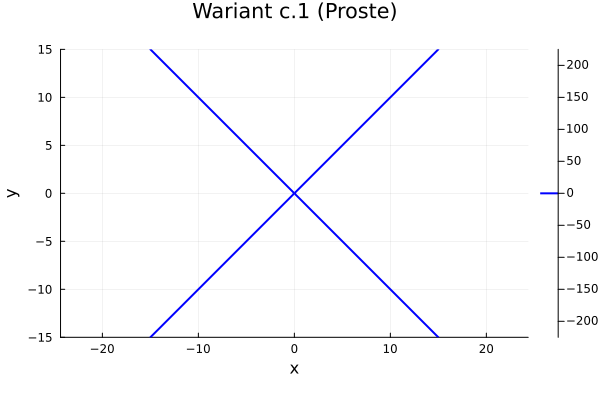
\includegraphics[width=0.5\textwidth]{plots/wykres_c1.png}
    \caption{Wizualizacja rozmaitości $V(I_f)$ dla wariantu 1.}
\end{figure}

\subsection{Wariant 2: $f(x,y,z) = z - 8$}
\textbf{Wynik z programu:} $\{-x^2 + y^2 + 64.0, \, z - 8.0, \, x^2 - y^2 - z^2\}$ \\
\textbf{Wyznaczenie ideału:} Eliminując $z$ otrzymujemy $I_f = \langle x^2 - y^2 - 64 \rangle$. \\
\textbf{Uzasadnienie geometryczne:} Jest to klasyczna \textbf{hiperbola} o osi rzeczywistej wzdłuż osi X. Przecięcie stożka płaszczyzną poziomą $z=8$ (równoległą do podstawy) generuje krzywą stożkową będącą hiperbolą.


\begin{figure}[H]
    \centering
    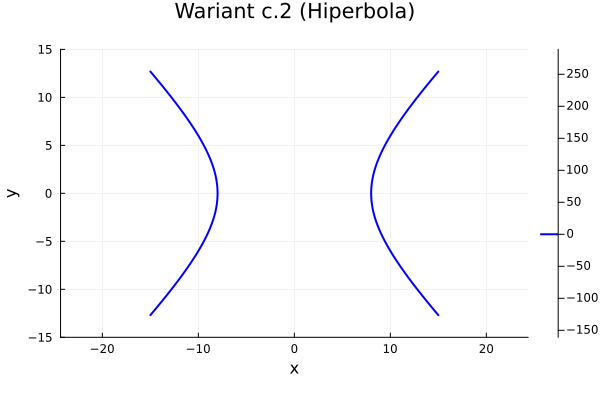
\includegraphics[width=0.5\textwidth]{plots/wykres_c2.png}
    \caption{Wizualizacja rozmaitości $V(I_f)$ dla wariantu 2.}
\end{figure}

\subsection{Wariant 3: $f(x,y,z) = x - z + 1$}
\textbf{Wynik z programu:} $\{2.0x + y^2 + 1.0, \, x - z + 1.0, \, x^2 - y^2 - z^2\}$ \\
\textbf{Wyznaczenie ideału:} Z bazy odczytujemy $I_f = \langle y^2 + 2x + 1 \rangle$. \\
\textbf{Uzasadnienie geometryczne:} Przekształcając równanie otrzymujemy $x = -\frac{1}{2}y^2 - \frac{1}{2}$. Jest to \textbf{parabola} skierowana ramionami w lewą stronę osi X. Powstaje ona, ponieważ płaszczyzna tnąca $z = x + 1$ jest ściśle równoległa do tworzącej stożka.

\begin{figure}[H]
    \centering
    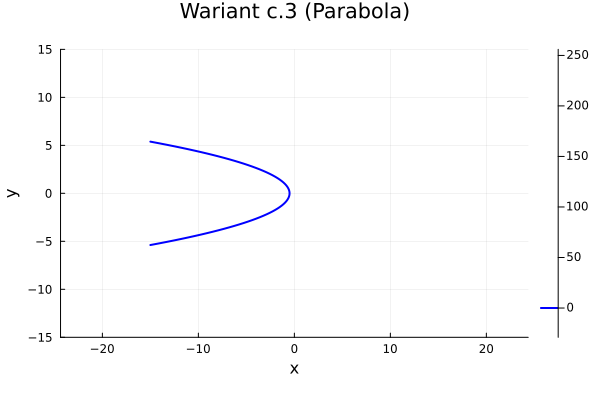
\includegraphics[width=0.5\textwidth]{plots/wykres_c3.png}
    \caption{Wizualizacja rozmaitości $V(I_f)$ dla wariantu 3.}
\end{figure}

\subsection{Wariant 4: $f(x,y,z) = x - y - z - 7$}
\textbf{Wynik z programu:} $\{-2.0xy - 14.0x + 2.0y^2 + 14.0y + 49.0, \, \dots\}$ \\
\textbf{Wyznaczenie ideału:} Wyeliminowany wielomian definiuje generator $I_f = \langle 2y^2 - 2xy - 14x + 14y + 49 \rangle$. \\
\textbf{Uzasadnienie geometryczne:} Obecność mieszanego członu $-2xy$ wskazuje na \textbf{hiperbolę ukośną} (obróconą względem osi układu współrzędnych). Wynika to z faktu, że płaszczyzna tnąca przecina obie części stożka pod kątem niesymetrycznym do jego głównych osi obrotu.

\begin{figure}[H]
    \centering
    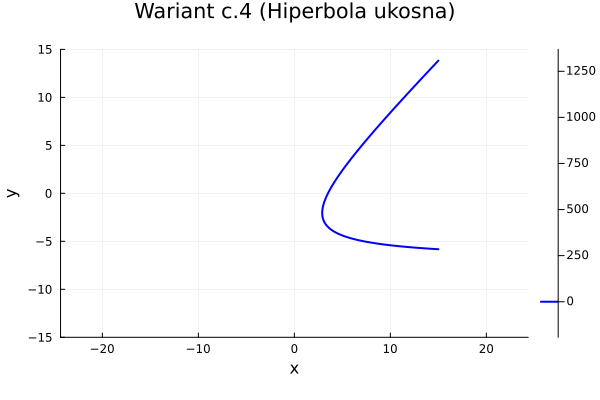
\includegraphics[width=0.5\textwidth]{plots/wykres_c4.png}
    \caption{Wizualizacja rozmaitości $V(I_f)$ dla wariantu 4.}
\end{figure}

\subsection{Wariant 5: $f(x,y,z) = 0.5y - z - 1$}
\textbf{Wynik z programu:} $\{-x^2 + 1.25y^2 - y + 1.0, \, \dots\}$ \\
\textbf{Wyznaczenie ideału:} Mnożąc wynik programu przez $-4$, otrzymujemy czystą postać algebraiczną: $I_f = \langle 4x^2 - 5y^2 + 4y - 4 \rangle$. \\
\textbf{Uzasadnienie geometryczne:} Przeciwne znaki przy współczynnikach $x^2$ (dodatni) oraz $y^2$ (ujemny) jednoznacznie definiują \textbf{hiperbolę} ze środkiem przesuniętym wzdłuż osi Y z powodu obecności składnika liniowego $+4y$.

\begin{figure}[H]
    \centering
    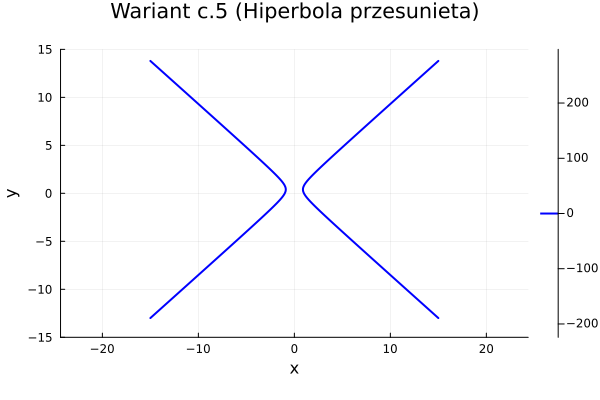
\includegraphics[width=0.5\textwidth]{plots/wykres_c5.png}
    \caption{Wizualizacja rozmaitości $V(I_f)$ dla wariantu 5.}
\end{figure}

% \begin{figure}[htbp]
    % \centering
    %\includegraphics[width=0.5\textwidth]{warianty_c.png}
    % \caption{Wizualizacja rozmaitości $V(I_f)$ dla wariantów 1-5 (wykresy wygenerowane zewnętrznie).}
% \end{figure}

\section{Układ wyższych rzędów i eliminacja zmiennej (Punkt d)}
Rozważamy układ:
$\begin{cases}
(x^2 - y^2 + 2x)^2 = z^2(x^2 - y^2) \\
x - 2y - 3z = 0
\end{cases}$

\subsection{Eliminacja zmiennej $x$}
Zgodnie z wykonanym testem, program dla porządku leksykograficznego wypluł wielomian eliminacyjny niezależny od $x$:
\[ 9y^4 + 72y^3z + 24y^3 + 195y^2z^2 + 132y^2z + 16y^2 + 204yz^3 + 216yz^2 + 48yz + 72z^4 + 108z^3 + 36z^2 = 0 \]
Wykres tego równania w zmiennych $(y,z)$ przedstawia algebraiczną krzywą rzutu na płaszczyznę YZ, posiadającą izolowane punkty osobliwe wynikające z geometrii przecięcia kwartyki z płaszczyzną.

\begin{figure}[H]
    \centering
    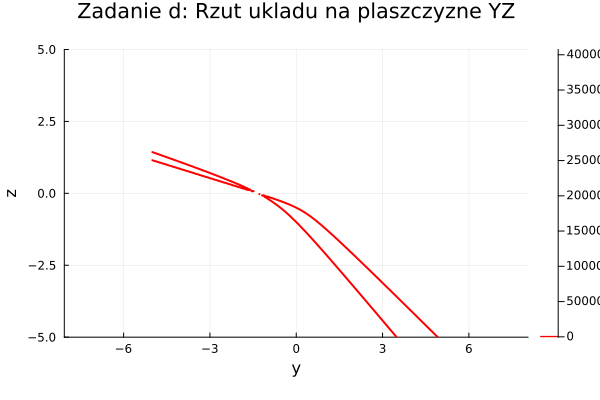
\includegraphics[width=0.5\textwidth]{plots/wykres_d1.png}
    \caption{Wykres rozwiązania układu w zmiennych y i z (rzut na płaszczyznę YZ).}
\end{figure}

\subsection{Analiza przekroju dla $z=2$}
Podstawiając stałą $z = a = 2$ do pierwszego równania układu, otrzymujemy:
\[ (x^2 - y^2 + 2x)^2 = 4(x^2 - y^2) \]

Wykres tego równania na płaszczyźnie XY tworzy krzywą algebraiczną czwartego stopnia zwaną \textbf{krzywą gruszkowatą} (ang. \textit{piriform curve}, lub zniekształconą lemniskatą). Posiada ona charakterystyczny węzeł (samoprzecięcie) w początku układu współrzędnych $(0,0)$, co jest bezpośrednią konsekwencją zerowania się składników niższych rzędów w tym punkcie.

\begin{figure}[H]
    \centering
    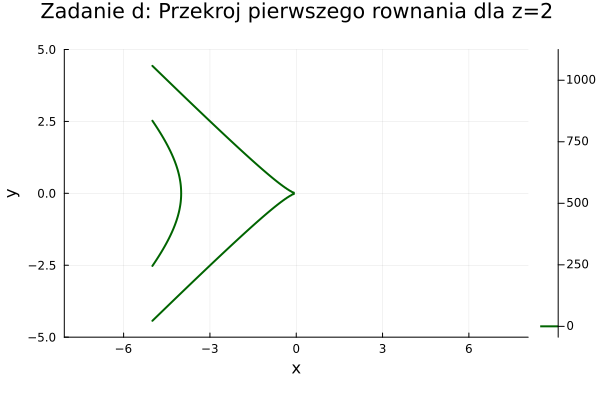
\includegraphics[width=0.5\textwidth]{plots/wykres_d2.png}
    \caption{Wykres rozwiązania pierwszego równania układu w zmiennych x i y, dla z = 2.}
\end{figure}

\section{Wyznaczanie wzoru trysektrysy (Punkt e)}
Trysektrysa we współrzędnych biegunowych zadana jest jako:
\[ r = 7\frac{4\cos\theta - 1}{\cos\theta} \]

\subsection{Przejście do współrzędnych kartezjańskich za pomocą Bazy Groebnera}
Do programu wprowadzono układ powiązany z definicją zmiany układu współrzędnych ($z$ reprezentuje promień $r$):
1) Relacja biegunowa po wymnożeniu: $zx + 7z - 28x = 0$ \\
2) Definicja promienia: $z^2 - x^2 - y^2 = 0$

Wykonanie algorytmu Buchbergera zwróciło wielomian eliminacyjny czwartego stopnia:
\[ -0.00510204x^4 - 0.07142857x^3 - 0.00510204x^2y^2 + 3.75x^2 - 0.07142857xy^2 - 0.25y^2 = 0 \]
Mnożąc całe równanie przez $-196$ (gdyż $0.00510204 \approx \frac{1}{196}$), uzyskujemy dokładną postać całkowitoliczbową:
\[ x^4 + 14x^3 + x^2y^2 - 735x^2 + 14xy^2 + 49y^2 = 0 \]
Krzywa ta posiada pętlę przechodzącą przez środek układu oraz dwa ramiona dążące do asymptoty pionowej $x = -7$.

\begin{figure}[H]
    \centering
    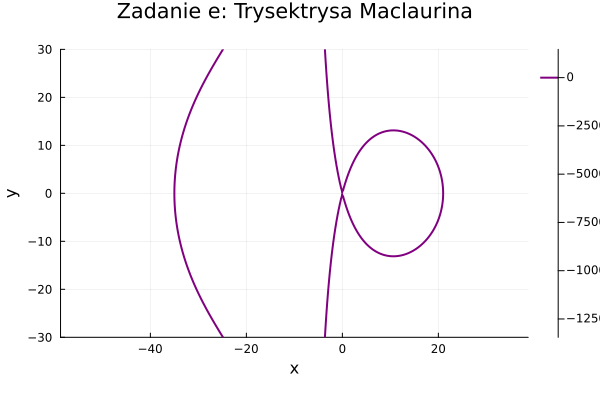
\includegraphics[width=0.5\textwidth]{plots/wykres_e.png}
    \caption{Wizualizacja Trysektrysy.}
\end{figure}

\subsection{Zjawisko numeryczne w punkcie (e)}
Wydruk z bazy Groebnera zawierał końcowe linie typu $1.16\times 10^{-10}x^2$ oraz $-49.0y^2$. Jest to klasyczny przejaw \textbf{niestabilności numerycznej algorytmu Buchbergera} wywołanej stosowaniem arytmetyki zmiennoprzecinkowej ($\tt{Float64}$). W wyniku wielokrotnych dzieleń i odejmowań współczynników, wartości, które teoretycznie powinny wynosić zero, osiągnęły małe wartości niezerowe (błąd zaokrągleń maszynowych). Spowodowało to błędne uznanie tych reszt za nowe elementy bazy i wygenerowało zbędny "ogon" numeryczny.

\subsection{Zastosowanie trysektrysy}
Trysektrysa (w tym przypadku trysektrysa Maclaurina) to słynna krzywa wyższego stopnia wykorzystywana w geometrii klasycznej do rozwiązania problemu \textbf{trysekcji kąta} — czyli podziału dowolnego kąta na trzy równe części. Udowodniono, że operacja ta jest niewykonalna przy użyciu wyłącznie cyrkla i nieoznaczonej linijki. Jednakże przyzwolenie na konstrukcję z wykorzystaniem gotowej krzywej płaskiej (jaką jest trysektrysa) w pełni umożliwia dokładne i konstrukcyjne podzielenie dowolnego kąta.

\end{document}